\begin{document}
%Mapping the Higgs total width out from strong phases of the SM} 
\begin{center}{\it by John Campbell, Marcela Carena, Roni Harnik and Zhen Liu} \footnote{This manuscript has been authored by Fermi Research Alliance, LLC under Contract No. DE-AC02-07CH11359 with the U.S. Department of Energy, Office of Science, Office of High Energy Physics.}\end{center}


%\subsubsection*{Introduction.}

The SM Higgs total decay width can be constrained from the change in on-shell Higgs rates due to interference effects between the Higgs signal and the QCD background~\cite{Campbell:2017rke}. This change in rates requires the existence of a so-called strong phase in the amplitudes, that can be present both  in the Higgs signal and in the continuum background, as is the case in the SM. We shall demonstrate that,
the different scaling behaviour between   the strong phase induced interference  and the Breit-Wigner parts of the on-shell Higgs rate may allow the placement of bounds on, or even measurements of, the Higgs boson total width.
Both theoretical and experimental uncertainties are the leading  limiting factors in this program. On the other hand, without  the strong phase induced interference effects, fits to on-shell Higgs rates can only place bounds on the total width by making definite theoretical assumptions~\cite{Duhrssen:2004cv,LHCHiggsCrossSectionWorkingGroup:2012nn,Dobrescu:2012td}. 

%\label{sec:result}
It is useful to write the amplitude for $gg \to h \to \gamma\gamma$ in a form which explicitly factors out the loop-induced couplings to gluons
($F_{gg}$) and photons ($F_{\gamma\gamma}$),
\begin{equation}
A_h \equiv A_{gg\to h\to\gamma\gamma}  \propto \frac {\hat s} {\hat s-m_h^2+i\Gamma_h m_h} F_{gg} F_{\gamma\gamma} \,.
\label{eq:Ah}
\end{equation}
Both the Higgs couplings $F_{gg}$ and $F_{\gamma\gamma}$ as well as the background amplitude $A_\mathrm{bkg}$
receive absorptive contributions that arise from loops of particles that are sufficiently light to be on shell. 
The resulting induced phases are usually dubbed `strong phases' in the flavor literature and we will adopt this terminology here.\footnote{Strong phases, which are CP even, get their name because they often arise in flavor physics from QCD dynamics. This is in contrast with CP odd weak phases, e.g., the relative size of the Higgs couplings to $F\tilde F$ versus $FF$. 
%in Higgs physics.
% which are Lagrangian parameters. 
%A weak phase in Higgs physics, for example, would .
}
In the presence of a strong phase we can write the interference term as
\begin{eqnarray}
|\mathcal{M}_h|^2_\mathrm{int} &&\equiv 2 \Re[A_h A_\mathrm{bkg}^*]= 
\frac {2 |A_\mathrm{bkg}||F_{gg}||F_{\gamma\gamma}|} {(\hat s - m_h^2)^2+\Gamma_h^2 m_h^2} \label{eq:phase}\\
&&\!\!
\times \!\left[ (\hat s-m_h^2) \cos (\delta_\mathrm{bkg}-\delta_h) \!+ \!m_h\Gamma_h \sin (\delta_\mathrm{bkg}-\delta_h) \right]\!\!, \nonumber
\end{eqnarray}
where we have taken $\delta_h=\mathrm{arg}[ F_{gg}]+\mathrm{arg}[F_{\gamma\gamma}]$ and $\delta_\mathrm{bkg}=\mathrm{arg}[ A_\mathrm{bkg}]$ as the signal and background strong phases, respectively.
The first term in the square bracket is the contribution to the interference term that does not modify the overall rate upon integration over $\hat s$. The second term is the subject of this work and leads to a modified rate in the presence of a strong phase. For convenience, we define $|\mathcal{M}_h|^2_\mathrm{int}=\mathcal{R}_h^\mathrm{int}+\mathcal{I}_h^\mathrm{int}$ and $\delta_s=\delta_\mathrm{bkg}-\delta_h$ such that
\bea
\mathcal{R}_h^\mathrm{int}&\equiv& \frac {2|A_\mathrm{bkg}||F_{gg}||F_{\gamma\gamma}|} {(\hat s - m_h^2)^2+\Gamma_h^2 m_h^2} (\hat s-m_h^2) \cos \delta_s \nonumber \\
\mathcal{I}_h^\mathrm{int}&\equiv& \frac {2|A_\mathrm{bkg}||F_{gg}||F_{\gamma\gamma}|} {(\hat s - m_h^2)^2+\Gamma_h^2 m_h^2} m_h\Gamma_h \sin \delta_s.
\eea

\begin{figure}[htbp]
\begin{center}
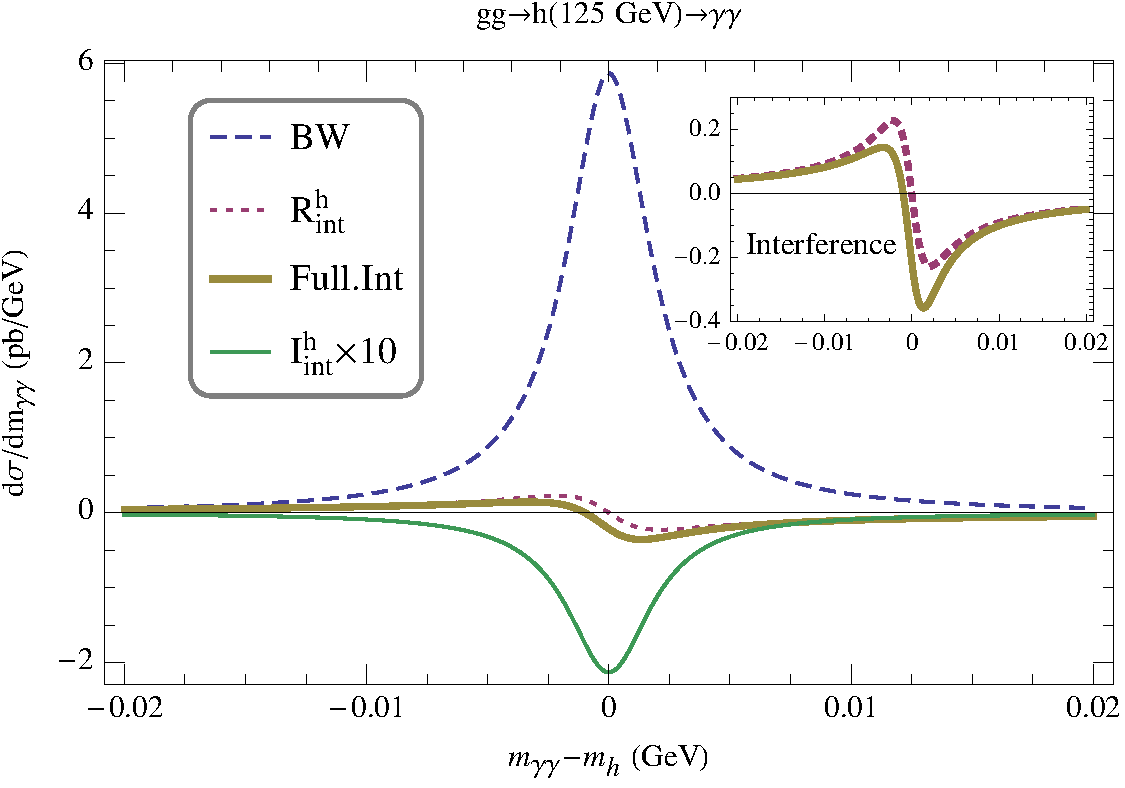
\includegraphics[scale=0.4,clip]{\main/section5/plots/signal_shape}
\caption{
The line-shape induced by various contributions to the cross-section for $gg \to h \to \gamma\gamma$ in the SM.
The Breit-Wigner line-shape, with no interference, is shown in blue (dashed) while the effect of $\mathcal{R}_h^\mathrm{int}$ and
$\mathcal{I}_h^\mathrm{int}$ (multiplied by a factor of 10) are shown in red (dotted) and green (solid), respectively.  The overall
effect of the interference in the full NLO calculation is given by the brown (solid) line. The insert in the top right is a magnification of the corresponding interference line-shapes.
}
\label{fig:sig_shape}
\end{center}
\vspace*{-0.6cm}
\end{figure}

In the SM the dominant contribution to $\mathcal{I}_h^\mathrm{int}$ comes from the phase of the background amplitude at two loops~\cite{Dicus:1987fk, Dixon:2003yb}. The signal amplitude also contains a
strong phase, mainly due to bottom quark loops. 
%For a detailed discussion, we refer the reader to appendices~\ref{sec:signalphase} and~\ref{sec:bkgphase}.  
We have performed a calculation of the interference effect that accounts for absorptive effects from both signal and background.
In Fig.~\ref{fig:sig_shape} we illustrate the features of the interference effects.
%For now we focus on the observable consequences of the interference, which we illustrate in Figure~\ref{fig:sig_shape}. 
The line shape, the differential cross-section as a function of~$\hat s$, is shown
for the pure Breit-Wigner (only $|A_h|^2$), and for the interference contributions $\mathcal{I}_h^\mathrm{int}$ and $\mathcal{R}_h^\mathrm{int}$ as well as for the sum of both. 
For visualisation, the interference contribution $\mathcal{I}_h^\mathrm{int}$ has been magnified by a factor of 10. 
%In this figure we have taken $\delta_h= (\pi+0.036)$ and $\delta_\mathrm{bkg}=-0.205$, obtained by averaging over different interfering helicity amplitudes up to two-loop order with virtual corrections alone. 
In this figure we show the line-shapes obtained including NLO effects with virtual corrections only. After summing over different interfering helicity amplitudes, we obtain averaged strong phases $\delta_h= (\pi+0.036)$ and $\delta_\mathrm{bkg}=-0.205$ for the signal and background, respectively.
%We obtain this figure by considering only virtual corrections up to two-loop order,
%\footnote{In the supplemental material we present details of a full NLO calculation and will find that the $\mathcal{I}_h^\mathrm{int}$ interference is destructive and results in about a 2\% reduction in the overall rate.}

As a concrete example that demonstrates the potential of this novel effect, without loss of generality
we can consider excursions in the flat direction corresponding to,
\be
\frac{|F_{gg}|^2|F_{\gamma\gamma}|^2}{|F^{\rm SM}_{gg}|^2|F^{\rm SM}_{\gamma\gamma}|^2}
 = \frac{\Gamma_h}{\Gamma^{\rm SM}_h} \,.
\label{eq:flatdir}
\ee
%If we define the two terms in the cross section in Eq.~(\ref{eq:sigma2}) as a Brieght-Wigner and an interference piece, $\sigma=\sigma_\mathrm{BW} + \sigma_\mathrm{int}$, 
The total Higgs cross section can then be written as,
\be
\sigma = \sigma_\mathrm{BW}^\mathrm{SM}\!\! \left(\!\!1\!+\! \frac {\sigma_\mathrm{int}^\mathrm{SM}} {\sigma_\mathrm{BW}^\mathrm{SM}}\sqrt{\frac {\Gamma_h} {\Gamma_h^\mathrm{SM}}}\right)
\simeq \sigma_\mathrm{BW}^\mathrm{SM} \!\!\left(\!\!1\!-\!2\%\sqrt{\frac {\Gamma_h} {\Gamma_h^\mathrm{SM}}}\right)\!\!.\label{eq:deltasigma}
\ee
%\bea
%\frac {\sigma_\mathrm{int}} {\sigma_\mathrm{BW}}&=& \frac {\sigma_{\rm int}^{\rm SM}} {\sigma_{\rm BW}^{\rm SM}} \, \sqrt{\Gamma_h/\Gamma_h^{\rm SM}}
% \nonumber \\
%& \simeq &  - 2\% \, \sqrt{\Gamma_h/\Gamma_h^{\rm SM}} \,.
%\label{eq:deltasigma}
%\eea
%
The result of a full NLO calculation of the interference effect are presented in Fig.~\ref{fig:width}, that shows the relative size of the interference effect as a function of the total width, normalised to its SM value, for parameter excursions defined by Eq.~(\ref{eq:flatdir}). 
\footnote{For details of the 
%full 
NLO calculation
%and discussion on the input paramters, kinematic distribution and decomposition of the interference effects
, see the supplemental material 
%of this work, which includes 
with Refs~\cite{Bern:1991aq,Bern:2001df,Bern:1995db,Bern:1993mq,Bern:2002jx,deFlorian:2013psa,Catani:1996vz,Campbell:2011bn,Dulat:2015mca,Djouadi:1997rj,Degrassi:2005mc,Passarino:2007fp,Dittmaier:2011ti}.}
The variation of the interference effect with the total width is shown imposing a 20~\UGeV $p_T^{h}$-veto, with and without LHC cuts on the final state photons. %(see next section for details). 
Since the interference effect is largest at small scattering angles, the photon cuts reduce the expected interference.  
This small consideration in the SM leads to much
bigger differences for $\Gamma_h \gg \Gamma_h^{\rm SM}$.
Observe that in the SM the interference contribution is destructive. However,  if the sign of $F_{gg} F_{\gamma\gamma}$ were flipped, ($\delta_s\to \pi+\delta_s$), the interference effect would lead to an enhancement of the di-photon rate rather than a suppression. 
The theoretical scale uncertainty is shown in the bottom panel of Fig.~\ref{fig:width} and amounts to about 
$^{+50\%}_{-30\%}$. For example, the interference effect is $-(2.20^{+1.06}_{-0.55})\%$ without photon cuts for SM Higgs.
%
\begin{figure}[htbp]
\begin{center}
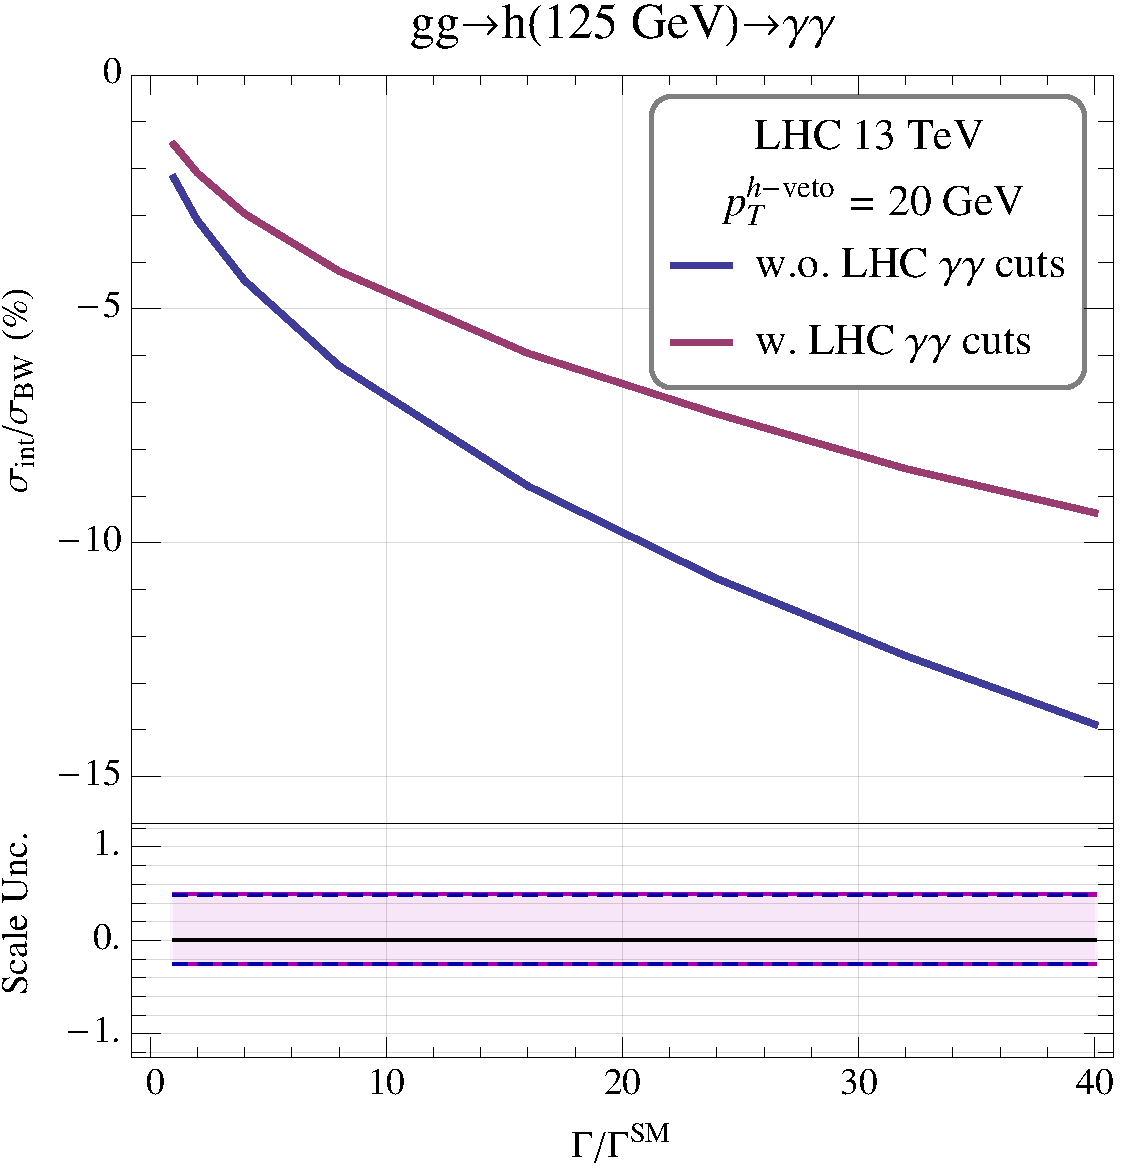
\includegraphics[scale=0.4,clip]{\main/section5/plots/widthdetermination_new}
\caption{
The total signal rate change due to the interference effect as a function of the Higgs total width normalised to its SM value, while keeping
the Breit-Wigner cross section identical to that of the SM Higgs. The magenta and blue (solid) lines represent the cases with and without LHC cuts
on the final state photons, respectively. The lower panel shows the scale variation uncertainties for these interference terms  as bands delimited by the blue (dashed)
 and magenta (solid) lines. The curves are obtained with a veto on the Higgs boson $p_T$  at 20 \UGeV. 
%\RH{add a space after the w. in the legend (or remove w.). add equal sign.}
}
\label{fig:width}
\end{center}

\end{figure}
%
Although a measurement at the 2\% level may be challenging at the LHC, 
this shows that a precise measurement of the $gg\to h \to \gamma\gamma$ rate can place a limit on the width of the Higgs boson. 
In this respect a measurement of the ratio of the $\gamma\gamma$ rate to the $4\ell$ rate is a promising route to reduce many of the systematic and theoretical, e.g. PDF and other parametric, uncertainties.

The best measured channels at the LHC, $gg\to h\to \gamma\gamma$ and $gg\to h \to 4\ell$, provide the most accurate cross section ratio, projected to 
 be measurable at the 4\% level~\cite{ATL-PHYS-PUB-2014-016}.   In contrast to single cross section measurements, the precision on this ratio is statistically limited.
Keeping the current theoretical uncertainty band in mind, the projected sensitivity of 4\% on the ratio of $\gamma\gamma$ to $4\ell$ yields
can be translated into an upper  limit of 22, 14, and 8 on $\Gamma_h/\Gamma_h^\mathrm{SM}$ at 1-$\sigma$ level, for low, central and high theoretical expectations
on this interference effect, respectively.\footnote{This limit is worse by one order of magnitude than the off-shell Higgs measurement that constrains the Higgs total width~\cite{Kauer:2012hd,Caola:2013yja,Campbell:2013una}. However, unlike the off-shell Higgs measurement, our effect is independent from the assumptions on the high-energy behaviour of the Higgs boson and the absence of new physics contribution in the off-shell region. 
%However, the off-shell constraint assumes that the Higgs couplings remain the same as the on-shell couplings and ignores any possible new physics contribution in the broad off-shell region. 
For more detailed discussion, see e.g., chapter I.8 of the Higgs Yellow Report~\cite{deFlorian:2016spz} and Refs.~\cite{Englert:2014aca,Logan:2014ppa}.} 
This assumes that the couplings to photons and $Z$ bosons maintain their SM ratio and the photon and gluon couplings respect Eq.~(\ref{eq:flatdir}).
The Higgs cross section precisions are anticipated to improve by a factor of three or so from statistical improvement at the HE-LHC with 27 \UTeV centre of mass energy and 15 $\fbi$ of integrated luminosity. %Using the same assumptions,  
This can be naively translated into  lower and upper limits on the Higgs total width of $\Gamma_h/\Gamma_h^\mathrm{SM}< 5$ at 1-$\sigma$ level using the central value from our NLO theory calculation. 
%This high level of precision may thus establish the existence of the interference effect at 3-$\sigma$ level and differential distribution study will further improve it.

In summary, we discuss the change in the $gg\to h\to \gamma\gamma$ on-shell rate, due to interference between the Higgs signal and the QCD background amplitudes, as a way to provide a novel handle to constrain - or even measure~-  the Higgs boson total width. 
We perform a full NLO calculation at order $\alpha_s^3$ of the interference effect and find that in the standard model it leads to a reduction of the on-shell rate by $\sim 2\%$. 
The proposed  method for gaining sensitivity to the Higgs boson width is complementary to other methods that have been discussed in the literature. 
Altogether our study aims at motivating  a more thorough examination of Higgs precision physics  taking into account the  strong phase induced interference effect in different Higgs boson observables.

\end{document}

